\begin{figure}
    \centering
    \subfigure[]{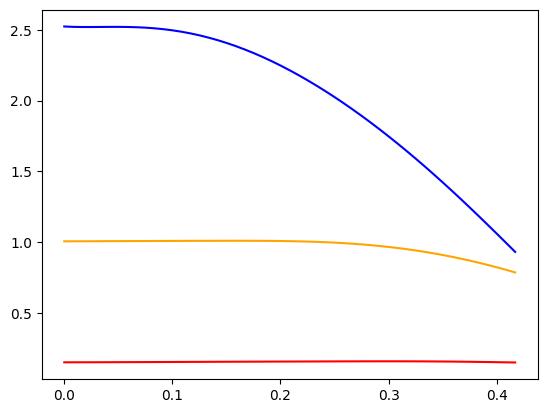
\includegraphics[width=0.3\columnwidth]{images/1.png}} 
    \subfigure[]{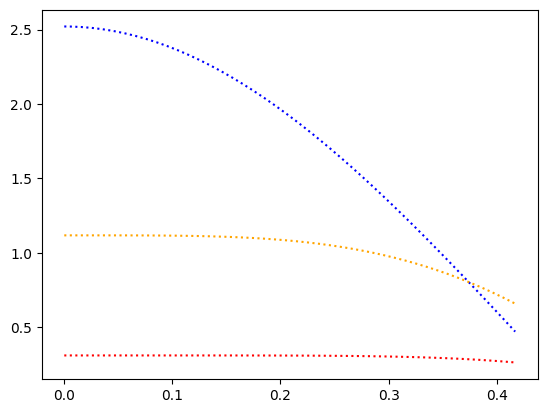
\includegraphics[width=0.3\columnwidth]{images/2.png}} 
    \subfigure[]{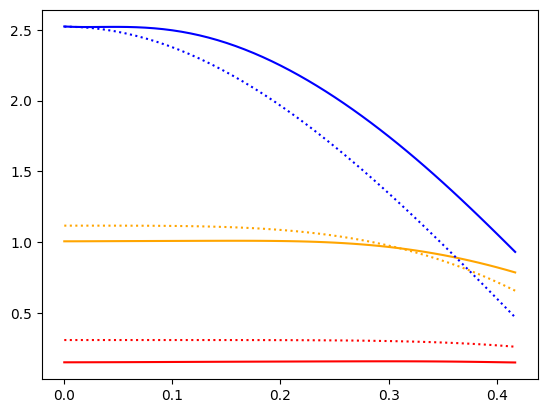
\includegraphics[width=0.3\columnwidth]{images/3.png}}
    \caption{(a) Resultados experimentais (b) Resultados teóricos (c) Comparação}
    \label{fig:foobar}
\end{figure}